
\section{Phase-Strategy Crossover Details}
\label{app:crossover-details}

On DeepSeek ($n{=}496$), a strategy ranking reversal emerges at $s{=}0.25$ (Figure~\ref{fig:crossover}): importance-based eviction yields \emph{lower} II than random in the high-sparsity phase ($0.021$ vs.\ $1.113$) but \emph{higher} II in the low-sparsity phase ($3.971$ vs.\ $1.514$---a $2.6{\times}$ reversal; both $p < 10^{-4}$). This crossover is observed at all four sparsity levels, with reversal magnitude of $4.0{\times}$ at $s{=}0.15$, $3.4{\times}$ at $s{=}0.20$, $2.6{\times}$ at $s{=}0.25$, and $2.2{\times}$ at $s{=}0.30$ (decreasing as random eviction severity rises). The reversal arises because head pruning redistributes attention mass, altering importance rankings in a way that couples the two sparsity mechanisms in low-sparsity phases (\S\ref{sec:discrimination-collapse-main}). Qwen does not exhibit a crossover: importance-based eviction produces lower II than random in both phases across all sparsity levels (e.g., at $s{=}0.25$: high $0.004$ vs.\ $1.108$; low $1.053$ vs.\ $1.769$).

\begin{figure}[t]
\centering
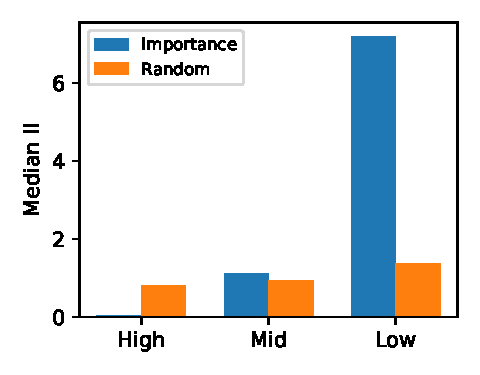
\includegraphics[width=\columnwidth]{fig3_crossover.pdf}
\caption{Strategy-dependent crossover at $s{=}0.25$ on DeepSeek ($n{=}496$). Grouped bar chart of median II by eviction strategy and reasoning phase. Importance-based eviction outperforms random in the high-sparsity phase but produces $2.6{\times}$ higher II in the low-sparsity phase, reversing the strategy ranking.}
\label{fig:crossover}
\end{figure}


\section{Profiling Subset Per-Phase Breakdown}
\label{app:profiling-subset}

\begin{table*}[t]
\centering
\small
\caption{Per-phase interaction index (II) from the $n{=}50$ profiling subset (DeepSeek-R1-Distill-Qwen-7B). This preliminary table does not include per-condition bootstrap CIs; full-scale values with bootstrap 95\% CIs ($B{=}10{,}000$) at $n{=}496$ appear in Table~\ref{tab:main-results}, and strategy-contrast CIs for this subset appear in the permutation test (Table~\ref{tab:permutation}). $G$ values use the ratio-of-medians definition ($\widetilde{\mathrm{II}}_{\textit{low}} / \widetilde{\mathrm{II}}_{\textit{high}}$) and serve as an auxiliary illustration of phase concentration; the primary evidence is $\Delta$ (see Appendix~\ref{app:g-metric}). At low sparsity ($s{=}0.15$), the ratio-of-medians and per-problem definitions diverge ($7.5{\times}$ vs.\ $69{\times}$) because per-problem ratios are sensitive to near-zero $\mathrm{II}_{\textit{high}}$ values.}
\label{tab:profiling-subset}
\begin{tabular}{@{}llccccr@{}}
\toprule
$s$ & Strategy & $\widetilde{\mathrm{II}}_{\textit{high}}$ & $\widetilde{\mathrm{II}}_{\textit{mid}}$ & $\widetilde{\mathrm{II}}_{\textit{low}}$ & $\Delta$ & $G$ \\
\midrule
0.15 & Importance & 0.006 & 0.081 & 0.398 & 0.39 & $\mathbf{69}$ \\
0.15 & Random     & 0.093 & 0.097 & 0.103 & 0.01 & 1.1 \\
\addlinespace
0.20 & Importance & 0.015 & 0.203 & 1.496 & 1.48 & $\mathbf{103}$ \\
0.20 & Random     & 0.292 & 0.350 & 0.276 & $-$0.02 & 0.9 \\
\addlinespace
0.25 & Importance & 0.032 & 1.118 & 7.196 & 7.16 & $\mathbf{222}$ \\
0.25 & Random     & 0.818 & 0.932 & 1.363 & 0.54 & 1.7 \\
\addlinespace
0.30 & Importance & 0.053 & 2.283 & 14.639 & 14.59 & $\mathbf{274}$ \\
0.30 & Random     & 2.503 & 2.592 & 4.041 & 1.54 & 1.6 \\
\bottomrule
\end{tabular}
\end{table*}

The $n{=}50$ profiling subset served as a preliminary calibration; all importance-based $\Delta$ values were subsequently replicated at $n{=}496$ with bootstrap 95\% CIs excluding zero (Table~\ref{tab:main-results}: $\Delta{=}0.39$\;$[0.35,\;0.44]$ to $8.48$\;$[7.75,\;9.69]$). The paired permutation test on this subset ($n{=}49$; Table~\ref{tab:permutation}) provides bootstrap 95\% CIs for the strategy contrast ($\widetilde{\Delta}_{\text{imp}} - \widetilde{\Delta}_{\text{rand}}$), all excluding zero after Bonferroni correction.


\section{Cross-Training-Paradigm Replication Details}
\label{app:cross-model-details}

Both models share the Qwen2ForCausalLM backbone (28 layers, 28 heads, 4-group GQA) but differ in training: DeepSeek uses reasoning distillation from DeepSeek-R1, while Qwen2.5 uses standard instruction tuning without explicit reasoning delimiters. This within-architecture-family comparison enables assessment of training methodology effects on the compound sparsity interaction, though causal attribution is limited by the observational design.

Despite lacking explicit \texttt{<think>} delimiters, Qwen2.5-7B-Instruct exhibits sufficient variation in attention sparsity to permit phase segmentation via the same quantile-based method (\S\ref{par:phase-segmentation}). Twenty-five of the 500 problems are excluded due to degenerate phase assignments, yielding $n{=}475$ valid problems for Qwen (vs.\ $n{=}496$ for DeepSeek).

\paragraph{Per-phase effective sample size.}
\label{app:qwen-null-rate}
Table~\ref{tab:qwen-effective-n} reports the per-phase effective sample size for Qwen2.5-7B-Instruct, defined as the number of problems with non-null phase segments (segment length $\geq$ \texttt{min\_phase\_length}). The mid-phase null rate (45.2\%) reflects problems where mid-sparsity tokens do not form contiguous runs above the merging threshold; this does not affect the low--high contrast ($\Delta$) used in the primary analysis.

\begin{table}[t]
\centering
\small
\caption{Per-phase effective sample size for Qwen2.5-7B-Instruct ($n_{\text{eff}} = 475$). Phase segmentation is performed once on dense-model attention patterns and is independent of sparsity level.}
\label{tab:qwen-effective-n}
\begin{tabular}{@{}lcccc@{}}
\toprule
Phase & $s{=}0.15$ & $s{=}0.20$ & $s{=}0.25$ & $s{=}0.30$ \\
\midrule
High & 475 & 475 & 475 & 475 \\
Mid  & 274 & 274 & 274 & 274 \\
Low  & 475 & 475 & 475 & 475 \\
\bottomrule
\end{tabular}
\end{table}

Table~\ref{tab:cross-model} reports the cross-training-paradigm comparison. Qwen reproduces the monotonic severity gradient at ${\sim}1/5$ of DeepSeek's magnitude. Figure~\ref{fig:cross-model} visualizes this comparison.

\begin{table}[t]
\centering
\small
\caption{Cross-training-paradigm comparison of median compound severity difference ($\Delta$) under importance-based eviction.}
\label{tab:cross-model}
\begin{tabular}{@{}lcccc@{}}
\toprule
Model & $s{=}0.15$ & $s{=}0.20$ & $s{=}0.25$ & $s{=}0.30$ \\
\midrule
DeepSeek-R1-Distill-Qwen-7B ($n{=}496$) & 0.39 & 1.21 & 3.99 & 8.48 \\
Qwen2.5-7B-Instruct ($n{=}475$)         & 0.07 & 0.31 & 1.07 & 3.16 \\
\bottomrule
\end{tabular}
\end{table}

\begin{figure}[t]
\centering
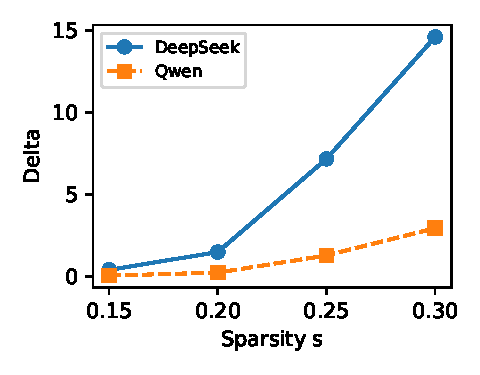
\includegraphics[width=\columnwidth]{fig5_crossmodel.pdf}
\caption{Cross-training-paradigm comparison of the median severity difference under importance-based eviction ($n{=}496$/$475$). Both DeepSeek (solid) and Qwen (dashed) exhibit monotonically increasing $\Delta$ with sparsity; Qwen's magnitude is approximately one-quarter to one-sixth of DeepSeek's.}
\label{fig:cross-model}
\end{figure}

\paragraph{Per-problem concordance.}
The per-problem concordance across models is not significant (mean $\rho = -0.107$, $p = 0.926$), indicating that while the aggregate gradient direction replicates, the specific problems driving severity differ between models---consistent with model-specific attention patterns rather than a universal per-problem vulnerability ranking.

\paragraph{Random eviction control.}
As a control, random eviction on Qwen mirrors DeepSeek: non-significant at $s \leq 0.20$ ($\Delta$: $-0.01$, $0.02$; CIs span zero) but significant at $s \geq 0.25$ ($\Delta{=}0.39$, $p_{\text{Bonf}} < 10^{-10}$; $\Delta{=}0.91$, $p_{\text{Bonf}} < 10^{-13}$). Where significant, the random phase gradient is $2.7$--$3.5{\times}$ weaker than importance-based ($0.39$ vs.\ $1.07$ at $s{=}0.25$; $0.91$ vs.\ $3.16$ at $s{=}0.30$), supporting strategy-specific amplification.


\section{Permutation Test Details}
\label{app:permutation-details}

For each problem $i$ and sparsity level $s$, we compute the compound severity difference $\Delta_i^{(\text{strat})} = \mathrm{II}_{\textit{low},i} - \mathrm{II}_{\textit{high},i}$ under each eviction strategy. The test statistic is the median of the paired difference $\widetilde{\Delta} = \text{median}_i\!\bigl(\Delta_i^{(\text{imp})} - \Delta_i^{(\text{rand})}\bigr)$, measuring whether importance-based eviction produces systematically larger phase-dependent severity than random eviction. We permute strategy labels $10{,}000$ times to construct the null distribution and apply Bonferroni correction for 4 sparsity-level comparisons.

Per-problem distributions of the paired severity difference $\Delta_i = \mathrm{II}_{\textit{low},i} - \mathrm{II}_{\textit{high},i}$ under importance-based eviction are right-skewed at all sparsity levels, with mean/median ratios ranging from $1.2{\times}$ ($s{=}0.15$) to $1.6{\times}$ ($s{=}0.30$) for DeepSeek and $1.1{\times}$ to $1.4{\times}$ for Qwen.

The permutation null distributions are approximately symmetric around zero at all sparsity levels. At $s{=}0.15$, the observed statistic falls at the $99.92$th percentile of the null ($p_{\text{Bonf}} = 0.0032$); at $s \geq 0.20$, no permutation exceeds the observed statistic.

Table~\ref{tab:permutation} reports the results. All four sparsity levels reject $H_0$ after Bonferroni correction ($p_{\text{Bonf}} < 0.005$), with observed median differences increasing monotonically from $0.37$ at $s{=}0.15$ to $9.85$ at $s{=}0.30$. The monotonic growth of both the point estimate and the CI lower bound ($0.19 \to 0.69 \to 1.66 \to 6.70$) supports that compound severity amplification strengthens with sparsity---not merely in central tendency but also in worst-case lower bounds. Figure~\ref{fig:permtest-forest} presents these results as a forest plot.

\begin{table}[t]
\centering
\small
\caption{Paired permutation test for compound severity: importance vs.\ random eviction on DeepSeek-R1-Distill-Qwen-7B ($n{=}49$ profiling subset, $10{,}000$ permutations, Bonferroni-corrected). The monotonic $\Delta$ pattern is supported at $n{=}496$ (Table~\ref{tab:aggregate-ii}).}
\label{tab:permutation}
\begin{tabular}{@{}rrcl@{}}
\toprule
$s$ & Observed $\widetilde{\Delta}$ & 95\% CI & $p_{\text{Bonf}}$ \\
\midrule
0.15 & 0.37 & $[0.19,\; 0.62]$ & 0.0032 \\
0.20 & 0.97 & $[0.69,\; 1.49]$ & ${<}\,0.001$ \\
0.25 & 3.34 & $[1.66,\; 6.64]$ & ${<}\,0.001$ \\
0.30 & 9.85 & $[6.70,\; 16.29]$ & ${<}\,0.001$ \\
\bottomrule
\end{tabular}
\end{table}

\begin{figure}[t]
\centering
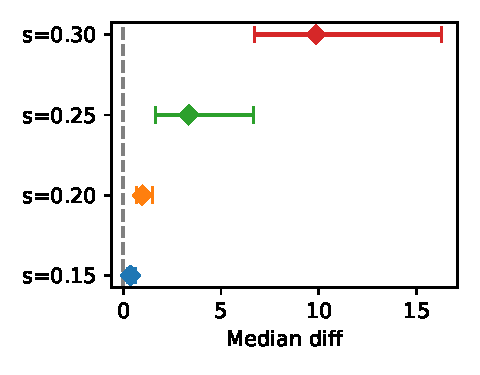
\includegraphics[width=\columnwidth]{fig4_bootstrap.pdf}
\caption{Forest plot of permutation test results. Horizontal bars show 95\% permutation CIs; diamonds mark observed median differences $\widetilde{\Delta}$. All CIs lie entirely above zero, supporting significant strategy-dependent severity at every sparsity level.}
\label{fig:permtest-forest}
\end{figure}


\section{Cross-Architecture Analysis}
\label{app:cross-arch}

To test whether the phase-modulated severity pattern extends beyond the Qwen2 architecture, we replicate the full experiment on DeepSeek-R1-Distill-Llama-8B (LlamaForCausalLM, 8B parameters; $n{=}250$, MATH-500) under both importance-based and random eviction at $s \in \{0.15, 0.20, 0.25, 0.30\}$. Table~\ref{tab:llama-cross-arch} reports paired median differences and effect sizes for all 8 conditions.

The within-importance phase gradient replicates with large effect sizes: $\Delta$ rises monotonically from $0.050$ ($s{=}0.15$, $d_z{=}0.81$) to $0.695$ ($s{=}0.30$, $d_z{=}1.15$), all $p < 10^{-29}$. An architecture-specific difference emerges in strategy specificity: random eviction on LLaMA also exhibits statistically significant phase gradients at all four sparsity levels ($\Delta{=}0.025$--$0.271$; $d_z{=}0.41$--$0.46$; all $p < 10^{-12}$), unlike DeepSeek and Qwen where random eviction is non-significant at $s \leq 0.20$. The importance/random $\Delta$ ratio on LLaMA is $2.0$--$2.6{\times}$, substantially weaker than the $15$--$17{\times}$ observed on DeepSeek.

Dose-response monotonicity holds for both strategies across all sparsity levels, supporting the phase gradient as an architecture-general phenomenon. The reduced strategy specificity on LLaMA suggests that GQA's grouped key-value structure partially preserves importance score quality under head pruning, attenuating the discrimination collapse that drives strategy divergence on MHA architectures.

\begin{table}[t]
\centering
\small
\caption{Cross-architecture validation: paired median difference ($\Delta$) and effect size ($d_z$) on DeepSeek-R1-Distill-Llama-8B (LlamaForCausalLM, $n{=}250$, MATH-500). All conditions are monotonic.}
\label{tab:llama-cross-arch}
\begin{tabular}{@{}llccc@{}}
\toprule
$s$ & Strategy & $\Delta$ & $d_z$ & $p$ \\
\midrule
0.15 & Importance & $0.050$ & $0.814$ & $1.4 \times 10^{-29}$ \\
0.15 & Random     & $0.025$ & $0.436$ & $9.3 \times 10^{-13}$ \\
\addlinespace
0.20 & Importance & $0.159$ & $1.010$ & $8.9 \times 10^{-35}$ \\
0.20 & Random     & $0.065$ & $0.459$ & $3.6 \times 10^{-15}$ \\
\addlinespace
0.25 & Importance & $0.376$ & $1.115$ & $4.3 \times 10^{-39}$ \\
0.25 & Random     & $0.184$ & $0.424$ & $3.8 \times 10^{-13}$ \\
\addlinespace
0.30 & Importance & $0.695$ & $1.150$ & $1.5 \times 10^{-40}$ \\
0.30 & Random     & $0.271$ & $0.410$ & $6.0 \times 10^{-12}$ \\
\bottomrule
\multicolumn{5}{@{}l}{\footnotesize Imp/Rand $\Delta$ ratio: $2.0$--$2.6{\times}$ (cf.\ $15$--$17{\times}$ on DeepSeek).}
\end{tabular}
\end{table}

\paragraph{Magnitude comparison.}
LLaMA interaction magnitudes are approximately $7$--$12{\times}$ smaller than Qwen2-architecture models at matched sparsity. This gap likely reflects differences in attention head specialization between MHA (Qwen2, 28 heads) and GQA (LLaMA, 32 heads with 8 KV groups). The phase gradient direction and dose-response monotonicity replicate, supporting the architecture-generality of phase-modulated compound interaction. Strategy specificity, however, is weaker ($2.0$--$2.6{\times}$ on LLaMA vs.\ $15$--$17{\times}$ on DeepSeek), indicating that the magnitude of strategy${\times}$phase interaction depends on architectural factors governing importance score stability under pruning.


\section{Analysis: Importance Discrimination Collapse}
\label{app:analysis}

\subsection{Importance Discrimination Collapse}
\label{sec:discrimination-collapse}

Head pruning reduces the number of heads contributing to cumulative importance scores, collapsing the score distribution. Table~\ref{tab:discrimination-metrics-full} quantifies this effect: the Gini coefficient decreases by $0.030$--$0.081$ (DeepSeek) and $0.010$--$0.020$ (Qwen) after pruning, with consistent negative deltas across all 16 conditions (both models $\times$ 4 sparsity levels $\times$ 2 strategies). The CV delta is likewise negative in all 8 importance-based conditions. The same pattern holds under random eviction, indicating that importance discrimination collapse is a consequence of head pruning \emph{per se}, not of the eviction strategy.

\begin{table}[t]
\centering
\caption{Importance discrimination collapse under importance-based eviction. $\Delta\mathrm{Gini}$ and $\Delta\mathrm{CV}$ are post-pruning minus baseline; negative values indicate reduced discriminative power.}
\label{tab:discrimination-metrics-full}
\small
\begin{tabular}{llrr}
\toprule
Model & $s$ & $\Delta\mathrm{Gini}$ & $\Delta\mathrm{CV}$ \\
\midrule
DeepSeek & $0.15$ & $-0.030$ & $-0.56$ \\
DeepSeek & $0.20$ & $-0.040$ & $-0.77$ \\
DeepSeek & $0.25$ & $-0.065$ & $-1.29$ \\
DeepSeek & $0.30$ & $-0.081$ & $-1.66$ \\
\midrule
Qwen & $0.15$ & $-0.010$ & $-0.05$ \\
Qwen & $0.20$ & $-0.012$ & $-0.21$ \\
Qwen & $0.25$ & $-0.010$ & $-1.49$ \\
Qwen & $0.30$ & $-0.020$ & $-1.14$ \\
\bottomrule
\end{tabular}
\end{table}

When importance scores lose discriminability, thresholding degenerates into noise-sensitive selection---functionally approaching biased random eviction. This is phase-dependent: in low-sparsity phases, attention is already broadly distributed, so pruning-induced collapse has maximum impact; in high-sparsity phases, concentration is preserved. Random eviction is immune because its decisions are independent of score quality, consistent with $G \approx 1$.

\subsection{Entropy Redistribution}
\label{sec:entropy-redistribution}

Beyond importance discrimination collapse, we examine whether head pruning also redistributes the attention entropy of surviving heads. We measure the mean attention entropy per head:
\begin{equation}
    \mathcal{H}_i^{(h)} = -\sum_{j=1}^{T} a_{ij}^{(h)} \log a_{ij}^{(h)}
    \label{eq:attn-entropy}
\end{equation}
and compute $\Delta\mathcal{H}$ as the change from baseline (no pruning) to the pruned condition.

For DeepSeek under importance-based eviction, the entropy delta is consistently negative across all four sparsity levels ($\Delta\mathcal{H} \in [-0.047, -0.040]$; Table~\ref{tab:entropy-deltas}), indicating that importance-based pruning systematically selects heads whose removal concentrates attention in the surviving heads, reinforcing importance discrimination collapse.

For Qwen, the entropy pattern only partially replicates. The delta is negative at $s{=}0.15$ ($\Delta\mathcal{H} = -0.073$) and $s{=}0.20$ ($-0.076$), consistent with DeepSeek. However, at $s{=}0.25$, the delta reverses to $+0.045$, with 22 of 30 problems showing positive entropy change. At $s{=}0.30$, the delta is near zero ($-0.007$). The $s{=}0.25$ reversal is systematic rather than a statistical artifact: it is consistent across all three reasoning phases (low: $+0.042$, mid: $+0.034$, high: $+0.017$). We interpret this as a genuine model-specific difference, possibly arising from distinct head specialization patterns: Qwen's instruction tuning (vs.\ DeepSeek's distillation-based training) may produce head configurations where removing 25\% of heads triggers compensatory broadening rather than concentration.

We characterize importance discrimination collapse as the robust, model-independent driver of the phase-strategy interaction, with entropy redistribution as a secondary amplifier that is consistent in DeepSeek but model-dependent in Qwen.

\begin{table}[t]
\centering
\caption{Attention entropy deltas ($\Delta\mathcal{H}$) under importance-based eviction. DeepSeek shows consistent entropy compression; Qwen partially replicates with a reversal at $s{=}0.25$.}
\label{tab:entropy-deltas}
\small
\begin{tabular}{llr}
\toprule
Model & $s$ & $\Delta\mathcal{H}$ \\
\midrule
DeepSeek & $0.15$ & $-0.040$ \\
DeepSeek & $0.20$ & $-0.047$ \\
DeepSeek & $0.25$ & $-0.045$ \\
DeepSeek & $0.30$ & $-0.044$ \\
\midrule
Qwen & $0.15$ & $-0.073$ \\
Qwen & $0.20$ & $-0.076$ \\
Qwen & $0.25$ & $+0.045$ \\
Qwen & $0.30$ & $-0.007$ \\
\bottomrule
\end{tabular}
\end{table}
